Первые версии языка SQL, тогда ещё называвшегося SEQUEL, были разработаны компанией IBM в рамках реализации реляционной СУБД
System R в 1974 году. SQL является стандартным языком для работы с реляционными базами данных и в настоящее время 
поддерживается практически всеми продуктами, представленными на рынке.

Официальный стандарт языка SQL был опубликован Американским национальным институтом стандартов (American National Standards Institute, ANSI) и Международной организацией по стандартизации (International Standards Organization, 150) в 1986 году, после чего был расширен в 1989 году, а затем "--- в 1992, 1999, 2003 и 2006 годах.

SQL является языком реляционных баз данных, поэтому он стал популярным тогда, когда популярной стала реляционная модель представления данных. Табличная структура реляционной базы данных со строками и столбцами интуитивно понятна пользователям, поэтому язык SQL является простым для изучения. 

Инструкции SQL похожи на обычные предложения английского языка, что упрощает их понимание. Частично это обусловлено тем, что инструкции SQL описывают данные, которые необходимо получить, а не способ их поиска.

Перечислим основные инструкции SQL:

\begin{enumerate}
    \item Выборка информации из базы данных с помощью инструкции SELECT. Можно извлечь все данные из таблицы или лишь часть из них, отсортировать их и получить итоговые значения, вычисляя суммы и средние величины.
    \item Изменение информации в базе данных. Инструкция INSERT добавляет данные, инструкция DELETE удаляет их, а инструкция UPDATE обновляет существующие данные.
    \item Создание и изменение базы данных путем определения структуры новых таблиц и удаления таблиц, ставших ненужными, для чего применяются инструкции CREATE И DROP.
\end{enumerate}

Также SQL используется для управления доступом к базе данных. С помощью инструкций SQL предоставляются и отменяются разного рода привилегии для различных пользователей. 

Пример запроса на языке SQL: 

SELECT CITY

    FROM OFFICES;

Ответом на данный запрос будут все данные из столбца CITY таблицы OFFICES (рис. \ref{fig:graph}) \cite{10}.
\begin{figure}[H]
    \centering
    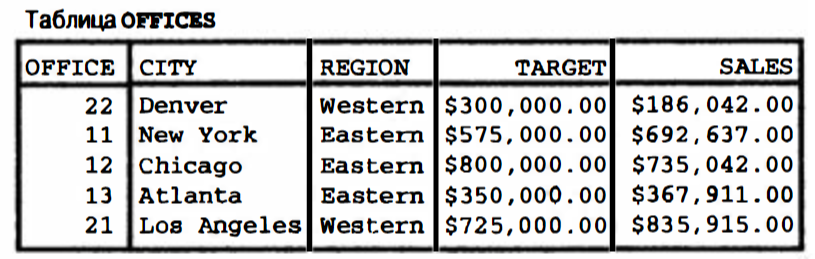
\includegraphics[width=0.7\textwidth]{offices.png}
    \caption{Простая реляционная база данных}
    \label{fig:graph}
\end{figure}

К плюсам языка SQL можно отнести его относительную простоту и низкий порог входа, универсальность, эффективность при работе с большими объемами данных. Также SQL имеет широкую поддержку и множество ресурсов для помощи при работе с языком.

Но одновременно с этим неопытному пользователю может быть достаточно сложно составить многоуровневый запрос. Сам SQL может иметь проблемы с производительностью при выполнении таких сложных запросов и с масштабированием на большие базы данных. А также при работе с SQL необходимо предпринимать дополнительные меры безопасности \cite{7}.